\documentclass[
	% -- opções da classe memoir --
	12pt,					% tamanho da fonte
	openright,				% capítulos começam em pág ímpar (insere página vazia caso preciso)
	twoside,					% para impressão em verso e anverso. Oposto a oneside
	a4paper,					% tamanho do papel. 
	% -- opções da classe abntex2 --
	%chapter=TITLE,			% títulos de capítulos convertidos em letras maiúsculas
	%section=TITLE,			% títulos de seções convertidos em letras maiúsculas
	%subsection=TITLE,		% títulos de subseções convertidos em letras maiúsculas
	%subsubsection=TITLE,	% títulos de subsubseções convertidos em letras maiúsculas
	% -- opções do pacote babel --
	english,					% idioma adicional para hifenização
	%french,					% idioma adicional para hifenização
	%spanish,				% idioma adicional para hifenização
	brazil					% o último idioma é o principal do documento
	]{abntex2}

% Silenciar warning memoir
\usepackage{silence}
\WarningFilter*{memoir}{You are using the caption package with the memoir class}

% ---------------------
% Pacotes OBRIGATÓRIOS
% ---------------------
\usepackage{lmodern}			% Usa a fonte Latin Modern			
\usepackage[T1]{fontenc}		% Seleção de códigos de fonte.
\usepackage[utf8]{inputenc}		% Codificação do documento (conversão automática dos acentos)
\usepackage{lastpage}			% Usado pela Ficha catalográfica
\usepackage{indentfirst}		% Identa o primeiro parágrafo de cada seção.
\usepackage{color}				% Controle das cores
\usepackage{graphicx,graphicx}	% Inclusão de gráficos
\usepackage{epsfig,subfig}		% Inclusão de figuras
\usepackage{microtype} 			% Melhorias de justificação
% ---------------------
		
% ---------------------
% Pacotes ADICIONAIS
% ---------------------
\usepackage{lipsum}						% Geração de dummy text
\usepackage{amsmath,amssymb,mathrsfs}	% Comandos matemáticos avançados 
\usepackage{setspace}  					% Para permitir espaçamento simples, 1 1/2 e duplo
\usepackage{verbatim}					% Para poder usar o ambiente "comment"
\usepackage{tabularx} 					% Para poder ter tabelas com colunas de largura auto-ajustável
\usepackage{afterpage} 					% Para executar um comando depois do fim da página corrente
\usepackage{url} 						% Para formatar URLs (endereços da Web)
% ---------------------

% ---------------------
% Pacotes de CITAÇÕES
% ---------------------
\usepackage[brazilian,hyperpageref]{backref}	% Paginas com as citações na bibl
% \usepackage[alf]{abntex2cite}					% Citações padrão ABNT (alfa)
\usepackage[num]{abntex2cite}					% Citações padrão ABNT (numéricas)
% ---------------------

% Configurações de CITAÇÕES para abntex2
% --- 
% CONFIGURAÇÕES DE PACOTES
% --- 

% ---
% Configurações do pacote backref
% Usado sem a opção hyperpageref de backref
\renewcommand{\backrefpagesname}{Citado na(s) página(s):~}
% Texto padrão antes do número das páginas
\renewcommand{\backref}{}
% Define os textos da citação
\renewcommand*{\backrefalt}[4]{
	\ifcase #1 %
		Nenhuma citação no texto.%
	\or
		Citado na página #2.%
	\else
		Citado #1 vezes nas páginas #2.%
	\fi}%
% ---

% Inclusão de dados para CAPA e FOLHA DE ROSTO (título, autor, orientador, etc.)
% ---
% Informações de dados para CAPA e FOLHA DE ROSTO
% ---
\titulo{Desenvolvimento e Análise de Viabilidade de Algoritmos de Detecção Facial}
\autor{Gabriel Pitali de Carvalho}
\newcommand{\imprimirautorinverso}{Carvalho, Gabriel Pitali de}
\local{Santo André}
\newcommand{\imprimirano}{2020}
\data{Abril de \imprimirano}
\orientador{André Kazuo Takahata}
\instituicao{Universidade Federal do ABC}
\newcommand{\imprimircurso}{Engenharia de Informação}
\newcommand{\imprimircentro}{Centro de Engenharia, Modelagem e Ciências Sociais Aplicadas}
\newcommand{\imprimirtrabalho}{Trabalho de Graduação em Engenharia de Informação}
\tipotrabalho{Monografia (Graduação - \imprimircurso)}
% O preambulo deve conter o tipo do trabalho, o objetivo,
% o nome da instituição e a área de concentração
\preambulo{\textbf{Trabalho de Graduação} apresentado ao concluir a Graduação em Engenharia de Informação, como parte dos requisitos necessários para a obtenção do Título Bacharel em Engenharia de Informação.}
% ---

% Inclui Configurações de aparência do PDF Final
%  Configurações de aparência do PDF final
% NÃO ALTERAR!!!

% alterando o aspecto da cor azul
\definecolor{blue}{RGB}{41,5,195}

% informações do PDF
\makeatletter
\hypersetup{
     	%pagebackref=true,
		pdftitle={\@title}, 
		pdfauthor={\@author},
    		pdfsubject={\imprimirpreambulo},
	    pdfcreator={LaTeX with abnTeX2},
		pdfkeywords={abnt}{latex}{abntex}{abntex2}{trabalho acadêmico}, 
		colorlinks=true,       		% false: boxed links; true: colored links
    		linkcolor=blue,          	% color of internal links
    		citecolor=blue,        		% color of links to bibliography
    		filecolor=magenta,      		% color of file links
		urlcolor=blue,
		bookmarksdepth=4
} 
\makeatother
% --- 

% O tamanho da identação do parágrafo é dado por:
\setlength{\parindent}{1.3cm}

% Controle do espaçamento entre um parágrafo e outro:
\setlength{\parskip}{0.2cm}  % tente também \onelineskip

% ---------------------
% Compila o índice
% ---------------------
\makeindex
% ---------------------

%%%%%%%%%%%%%%%%%%%%%%%%%%%
%%  INICIO DO DOCUMENTO  %%
%%%%%%%%%%%%%%%%%%%%%%%%%%%
\begin{document}

% Retira espaço extra obsoleto entre as frases.
\frenchspacing

% ----------------------------------------------------------
% ELEMENTOS PRÉ-TEXTUAIS (Capa, Resumo, Abstract, etc.)
% ----------------------------------------------------------
\pretextual

% Capa
% ---
% Impressão da Capa
% ---
  \begin{capa}%
    \center
	\ABNTEXchapterfont\large{Universidade Federal do ABC \\ Centro de Engenharia, Modelagem e Ciências Sociais Aplicadas \\ Trabalho de Graduação em Engenharia de Informação}
	%\vspace{1.5cm}

    \vfill
    \ABNTEXchapterfont\bfseries\LARGE\imprimirtitulo
    \vfill

	%\vfill
	\ABNTEXchapterfont\large\imprimirautor
	\vfill
%
	Número de Ordem : XXXX
	
    \large\imprimirlocal, \large\imprimirdata

    \vspace*{1cm}
  \end{capa}
% ---

% % Folha de rosto (o * indica que haverá a ficha bibliográfica)
\imprimirfolhaderosto*

% % Imprimir Ficha Catalográfica
% % ---
% Ficha Catalográfica
% ---
% Isto é um exemplo de Ficha Catalográfica, ou ``Dados internacionais de
% catalogação-na-publicação''. Você pode utilizar este modelo como referência. 
% Porém, talvez a biblioteca lhe fornece um PDF
% com a ficha catalográfica definitiva após a defesa do trabalho. Quando estiver
% com o documento, salve-o como PDF no diretório do seu projeto e substitua todo
% o conteúdo de implementação deste arquivo pelo comando abaixo:
%
% \begin{fichacatalografica}
%     \includepdf{fig_ficha_catalografica.pdf}
% \end{fichacatalografica}
\begin{fichacatalografica}
	\vspace*{\fill}					% Posição vertical
	\hrule							% Linha horizontal
	\begin{center}					% Centralizado
	\begin{minipage}[c]{12.5cm}		% Largura
	
	\imprimirautorinverso
	
	\hspace{0.5cm} \imprimirtitulo. / \imprimirautor. --
	\imprimirlocal.- \imprimirano.
	
	\hspace{0.5cm} \pageref{LastPage} p. : il.
	\bigbreak
	\hspace{0.5cm} \imprimirtipotrabalho~--~\imprimirinstituicao, \imprimirano.

	\hspace{0.5cm} \imprimirorientadorRotulo~\imprimirorientador
	\bigbreak
	\hspace{0.5cm} Bibliografia
	\bigbreak
	\hspace{0.5cm}
		1. Aprendizado de Máquina.
		2. Detecção Facial.
		I. \imprimirtitulo.
		II. \imprimirinstituicao
	\bigbreak
	\end{minipage}
	\end{center}
	\hrule
\end{fichacatalografica}
% ---

% % Inserir Folha de Aprovação
% % ---
% Assinaturas
% ---
% Isto é um exemplo de Folha de aprovação, elemento obrigatório da NBR
% 14724/2011 (seção 4.2.1.3). Você pode utilizar este modelo até a aprovação
% do trabalho. Após isso, substitua todo o conteúdo deste arquivo por uma
% imagem da página assinada pela banca com o comando abaixo:
%
% \includepdf{folhadeaprovacao_final.pdf}
%
\begin{folhadeaprovacao}

  \begin{center}
    {\ABNTEXchapterfont\large\imprimirautor}

    \vspace*{\fill}\vspace*{\fill}
    \begin{center}
      \ABNTEXchapterfont\bfseries\Large\imprimirtitulo
    \end{center}
    \vspace*{\fill}
    
    \hspace{.45\textwidth}
    \begin{minipage}{.5\textwidth}
        \imprimirpreambulo
    \end{minipage}%
    \vspace*{\fill}
   \end{center}
        
 % Isso na versao final do trabalho!!!       
   Trabalho aprovado. \imprimirlocal, 01 de janeiro de 2014:

   \assinatura{\textbf{\imprimirorientador} \\ Orientador} 
   \assinatura{\textbf{\imprimircoorientador} \\ Co-Orientador} 
   \assinatura{\textbf{Professor} \\ Convidado 1}
   \assinatura{\textbf{Professor} \\ Convidado 2}
   \assinatura{\textbf{Professor} \\ Convidado 3}
      
   \begin{center}
    \vspace*{0.5cm}
    {\large\imprimirlocal}
    \par
    {\large\imprimirdata}
    \vspace*{1cm}
  \end{center}
  
\end{folhadeaprovacao}
% ---

% % Dedicatória
% % ---
% Dedicatória
% ---
\begin{dedicatoria}
   \vspace*{\fill}
   \centering
   \noindent
   \textit{ Aos verme que roeu as frias carnes de meu cadáver.} \vspace*{\fill}
\end{dedicatoria}
% ---

% % Agradecimentos
% % ---
% Agradecimentos
% ---
\begin{agradecimentos}



Agradeço a Xuxa, meus pais, cachorro, gato e papagaio, por ...

Agradeço ao meu orientador, XXXXXXXXX, por todos os conselhos, pela paciência e ajuda nesse período.

Aos meus amigos ...

Aos professores ...

À XXXXXX pelo apoio financeiro para realização deste trabalho de pesquisa.

\end{agradecimentos}
%% ---

% % Epígrafe
% % ---
% Epígrafe
% ---
\begin{epigrafe}
    \vspace*{\fill}
	\begin{flushright}
		\textit{``Não sei o que, \\
		          não sei o que,\\
                  não sei o que lá.''\\
		          (Autor Desconhecido)}
	\end{flushright}
\end{epigrafe}
% ---

% % Resumo e Abstract
% % ---
% RESUMOS
% ---

% RESUMO em português
\setlength{\absparsep}{18pt} % ajusta o espaçamento dos parágrafos do resumo
\begin{resumo}
  Devido aos grandes avanços na área de visão computacional, muitas ferramentas relacionadas ao assunto têm sido criadas, mas torna-se complexo escolher qual a ideal para a necessidade existente e como podem ser aplicadas. Para entender melhor as opções disponíveis e suas aplicações, este trabalho apresenta um estudo sobre o desempenho de dois diferentes algoritmos de detecção facial em imagens e a análise da viabilidade da aplicação dos mesmos em um projeto comercial. Foi estudado o método de Viola-Jones de análise de características e uma \textit{rede neural convolucional em cascata multi tarefa} (MTCNN, \textit{Multi-Task Cascaded Convolutional Neural Network}) e o desempenho foi medido utilizando conjunto de imagens selecionado manualmente de acordo com uma lista de regras estabelecidas. A análise dos resultados foi feita em função da acurácia obtida e do lucro gerado pela aplicação de cada método em uma situação hipotética de uma empresa que necessita validar fotos cadastrais. Com o método de Viola-Jones foi demonstrado que é possível obter até \$0,136 de lucro por imagem analisada enquanto com o método MTCNN é possível ter o resultado mais lucrativo com \$0,142 de lucro por imagem analisada. Após a análise, foi possível determinar que é comercialmente interessante a implementação de modelos de visão computacional mas é necessário dedicar esforços para adequação das ferramentas aos objetivos específicos de cada caso.

  \textbf{Palavras-chaves}: Aprendizado de Máquina. Detecção Facial. Visão Computacional.
\end{resumo}

% ABSTRACT in english
\begin{resumo}[Abstract]
  \begin{otherlanguage*}{english}
    Due to the great advances in the field of computer vision, many tools related to this subject have been created, but it has become complex to choose which one is ideal for the existing needs and how they can be applied. In order to understand better the options available and their applications, this paper presents a study on the performance of two different face detection algorithms and the analysis of how feasible is to apply them in a commercial project. The Viola-Jones method of characteristic analysis and a Multi-Task Cascaded Convolutional Neural Network (MTCNN) were studied and their performances were measured using a set of manually selected images according to a list of established rules. The analysis of the results was made according to the accuracy obtained and the profit generated in a hypothetical situation of a company that needs to validate registration photos. It was demonstrated that Viola-Jones method can obtain up to \$0,136 profit per analyzed image while the MTCNN method can obtain the most profitable result with \$0,142 profit per analyzed image. After the analysis, it was possible to determine that it is commercially interesting to implement computer vision models, but it is necessary to dedicate efforts to adapt the tools to the specific objectives of each case.

    \vspace{\onelineskip}

    \noindent
    \textbf{Keywords}: Machine Learning. Face Detection. Computer Vision.
  \end{otherlanguage*}
\end{resumo}

% % Lista de ilustrações
% \pdfbookmark[0]{\listfigurename}{lof}
% \listoffigures*
% % \cleardoublepage

% % Lista de tabelas
% \pdfbookmark[0]{\listtablename}{lot}
% \listoftables*
% % \cleardoublepage

% % Lista de abreviaturas e siglas
% \begin{siglas}
%   \item[ABNT] Associação Brasileira de Normas Técnicas
%   \item[abnTeX] Normas para TeX
% \end{siglas}

% % Lista de símbolos
% \begin{simbolos}
%   \item[$ \Gamma $] Letra grega Gama
%   \item[$ \Lambda $] Lambda
%   \item[$ \zeta $] Letra grega minúscula zeta
%   \item[$ \in $] Pertence
% \end{simbolos}

% Inserir o SUMÁRIO
\pdfbookmark[0]{\contentsname}{toc}
\tableofcontents*
% \cleardoublepage

% ----------------------------------------------------------
% ELEMENTOS TEXTUAIS (Capítulos)
% ----------------------------------------------------------
\textual
% Elementos textuais com numeração arábica
\pagenumbering{arabic}
% Reinicia a contagem do número de páginas
\setcounter{page}{1}

% Inclui cada capitulo da Dissertação
% ----------------------------------------------------------
% Introdução 
% Capítulo sem numeração, mas presente no Sumário
% ----------------------------------------------------------

\chapter[Introdução]{Introdução}

Reconhecimento facial é uma tarefa trivial para humanos e a décadas tem sido um desafio para visão computacional e aprendizado de máquina. Desde os anos 90 o tema emerge em diferentes conferências e com o aumento do poder computacional dos dias atuais, sua capacidade se expande muito, fazendo com que tal assunto receba enorme atenção, principalmente devido ao seu grande valor comercial e as mais diversas aplicações possíveis, como verificação de identidade, controle de acesso, segurança, investigação de imagens em bancos de dados, vigilância, entretenimento ou realidade virtual \cite{appli2014} \cite{Zhao:2003:FRL:954339.954342}.

O processo de reconhecimento facial de forma automatizada é separado em quatro principais etapas, conforme detalhado no livro de \citeauthoronline{Li:2011:HFR:2073486} \cite{Li:2011:HFR:2073486}, primeiramente deve ser feita a \textit{detecção facial}, que consiste em validar e localizar a existência de alguma face na imagem ou vídeo, a segunda etapa consiste no \textit{alinhamento facial}, para que todas faces da base de dados sigam o mesmo padrão, a terceira etapa é a \textit{extração de características} que permite a obtenção de informação efetiva que será útil na distinção das diferentes faces, a quarta e última etapa consiste na \textit{correspondência de características}, onde as características extraídas anteriormente são comparadas com outras já conhecidas para que sejam identificadas.

Aprofundando o estudo da primeira etapa, de \textit{detecção facial}, \citeauthoronline{faceDetection2001} \cite{faceDetection2001} indica duas diferentes metodologias: a primeira baseada em características e a segunda baseada em imagens. Ambas posteriormente podem ser separadas em diversas técnicas mais específicas, como por exemplo a análise de características por constelação \cite{loy2006detecting} ou a análise de imagens com redes neurais \cite{cnn_face_detection}, onde cada técnica específica possui seus prós e contras em relação às demais.

\section{Objetivos e Motivação}

Este trabalho tem como objetivo encontrar uma forma eficiente de atuar sobre a primeira etapa (\textit{detecção facial}) do processo de reconhecimento facial, avaliando o desempenho qualitativo e quantitativo de diferentes metodologias e ferramentas disponíveis e permitindo a rápida identificação de imagens que não possuem uma face, para satisfazer a necessidade descrita a seguir.

Atualmente empresas e órgãos públicos possuem a necessidade de manter cadastros pessoais mas existe grande demanda para que estes cadastros sejam feitos de forma totalmente virtual pela população, pois isso evita o deslocamento de pessoas até os pontos de cadastro e torna todo o processo muito mais ágil. Certos cadastros incluem fotos de identificação e isto traz a necessidade de uma verificação feita por humanos para validar se a mesma consiste em uma foto de face frontal, conforme é necessário para o cadastro.

A validação citada já ocorre nas empresas e órgãos públicos que precisam coletar documentos de forma virtual e é frequentemente feita de forma totalmente manual, onde funcionários tem que verificar cada uma das imagens recebidas e muitas vezes se deparam com fotos sem nenhuma face frontal ou sem condições de serem identificadas (desfocadas, por exemplo), que são rejeitadas para que uma nova imagem seja solicitada. Estas imagens claramente inválidas por estarem em desacordo com o padrão esperado (foto de face frontal), poderiam ser eliminadas por uma filtragem anterior, reduzindo grande parte do trabalho que é feito hoje manualmente.

Portanto este trabalho demonstra como os métodos existentes atualmente para o processo de detecção facial poderiam ser aplicados nos processos expostos, adicionando uma etapa extra antes da validação manual e trazendo redução de custos para as empresas que necessitam de tal validação. Além de testar os métodos existentes, também é prosposto um modelo matemático que avalia a viabilididade e lucratividade de cada método a partir dos resultados dos testes.


% PARTE - Define a divisão do documento em partes (Não é obrigatório)
% \part{Preparação da pesquisa}
\chapter{Materiais e Métodos}\label{cap:ferramentas}

Com o objetivo de obter melhor entendimento sobre possíveis ferramenta de visão computacional e detecção facial, este trabalho descreve a execução de testes utilizando a linguagem de programação Python e a implementação da ferramenta OpenCV na mesma linguagem.

\section{OpenCV}

A ferramenta OpenCV, que pode ser encontrada no endereço \citeonline{itseez2015opencv}, é uma biblioteca de código aberto focada na solução de problemas utilizando visão computacional em tempo real, desenvolvida pela intel e posteriormente pela Itseez, com suporte a múltiplas plataformas e uso gratuito sobre a licença de código aberto BSD. A ferramenta apresenta suporte a frameworks de aprendizado profundo, como TensorFlow, Pytorch e Caffe e contempla tanto funções básicas, para aplicações como processamento de imagem, alteração de cor ou resolução, até aplicações avançadas, como detecção facial, identificação de características e biometria. \cite{wiki:OpenCV}

Neste trabalho, será utilizada a função de detecção de faces da ferramenta OpenCV, que utiliza um classificador em cascata baseado características, este é um método eficiente para reconhecimento de faces em imagens proposto por Paul Viola and Michael Jones, amplamente conhecido como método Viola-Jones, onde uma função é treinada com muitos exemplos positivos (imagens que contém o objeto a ser detectado) e negativos (imagens que não contém o objeto a ser detectado) e então utilizada para detectar as mesmas características em outras imagens. \cite{itseez2014theopencv}

A detecção de faces utilizando OpenCV consiste em duas etapas principais, o treinamento do modelo, onde são apresentadas diversas imagens já identificadas para que o modelo identifique padrões positivos e negativos. Após o treinamento, o modelo obtido pode ser utilizado para identificar, em novas imagens, características semelhantes as vistas nas imagens do treinamento. Neste projeto, será utilizado um modelo fornecido em conjunto com a ferramenta OpenCV, já treinado com diversos exemplos de faces frontais.

\section{Algoritmo Viola-Jones}

O algoritmo Viola-Jones foi publicado em 2001, no paper "Rapid object detection using a boosted cascade of simple features" ~\cite{paper-viola-jones} e é famoso por sua capacidade de detecção de faces com muita velocidade, isso ocorre devido a 3 principais técnicas utilizadas: o cálculo da imagem integral, o algoritmo de impulsão \textit{AdaBoost} e o classificador em cascata.

\subsection{Imagem Integral}

A primeira etapa do algoritmo Viola-Jones consiste em transformar a imagem original em uma imagem integral, isto é feito calculando o valor de cada pixel como a soma de todos os pixels que estão acima ou a esquerda do mesmo, como ilustrado na figura~\ref{fig:integral}.

\begin{figure}[htpb]
    \centering
    \caption{Imagem original (esquerda) e imagem integral (direita).}
    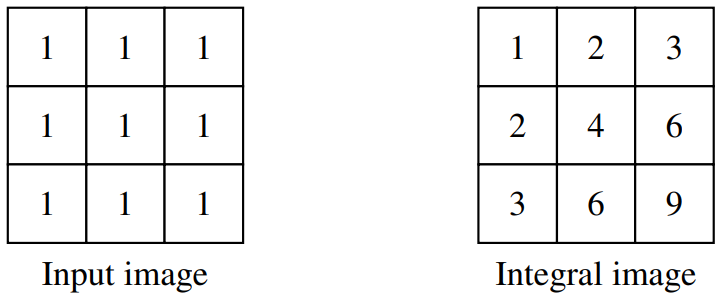
\includegraphics[scale=.4]{figs/imagem-integral.png}
    \legend{Fonte: \citeauthoronline{jensen2008implementingviolajones} (\citeyear{jensen2008implementingviolajones})}
    \label{fig:integral}
 \end{figure}

A utilização desta técnica permite calcular facilmente o tamanho de qualquer retângulo formado entre quatro pixels da imagem, conhecendo apenas o valor dos seus cantos, possibilitando assim a análise rápida de diversas partes da imagem. Tal calculo é feito definindo o retângulo a ser análisado e então aplicando a equação \ref{eq:img-integral}.

\begin{figure}[htb]
    \centering
    \caption{Representação da área da imagem a ser analisada.}
    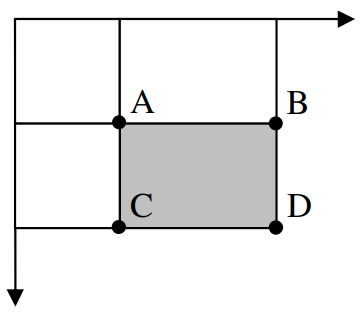
\includegraphics[scale=.4]{figs/imagem-integral-calculo.png}
    \legend{Fonte: \citeauthoronline{jensen2008implementingviolajones} (\citeyear{jensen2008implementingviolajones})}
    \label{fig:integral-calculo}
 \end{figure}

 \begin{equation}\label{eq:img-integral}
    \text{ Soma do retângulo cinza } = D - (B + C) + A
\end{equation}

Com a possibilidade de calcular facilmente a soma dos pixels de um retângulo arbitrário de forma rápida, o algoritmo para detecção pode analisar diversos trechos da imagem, chamados aqui de características, fazendo a comparação de duas ou mais áreas retângulares predefinidas, como os exemplos ilustrado na figura \ref{fig:features}. 

\begin{figure}[htb]
    \centering
    \caption{Alguns exemplos de características retângulares analisadas.}
    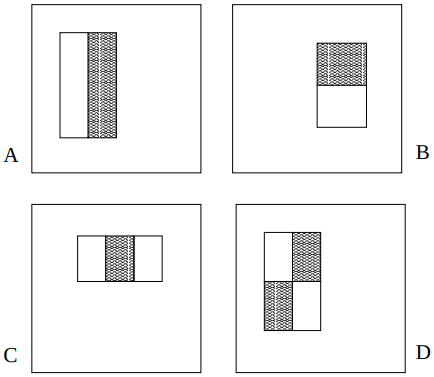
\includegraphics[scale=.5]{figs/features.png}
    \legend{Fonte: \citeauthoronline{paper-viola-jones} (\citeyear{paper-viola-jones})}
    \label{fig:features}
 \end{figure}

 O valor final de cada característica é definido pela soma do valor dos pixels sob o retângulo cinza menos a soma do valor dos pixels sob o retângulo branco.

%-
\subsection{Algoritmo de Impulsão AdaBoost}
%-

As características demonstradas anteriormente, são definidas basicamente como duas ou mais áreas retângulares de qualquer tamanho, tal simplicidade implica na possibilidade da criação de uma enorme variação das mesmas que precisariam ser calculadas diversas vezes, para cada parte de imagem e com diferentes tamanhos, isso implica em um alto custo de processamento, para evitar tal problema, durante a etapa de treinamento do modelo, é utilizado o algoritmo de impulsão \textit{AdaBoost}, que identifica quais são as características com maior probabilidade de acerto.

O \textit{AdaBoost}, que tem seu nome derivado de \textit{adaptative boosting} (traduzido como impulsão adaptativa), é um método de aprendizado de máquina que utiliza a combinação de vários classificadores fracos para obter uma classificação forte, no caso da detecção facial, o algoritmo é utilizado tanto para selecionar um conjunto de características mais eficientes como para treinar o classificador. \cite{fabio-luciana-2015}

\begin{figure}[htb]
    \centering
    \caption{Características retângulares mais eficientes para detecção facial.}
    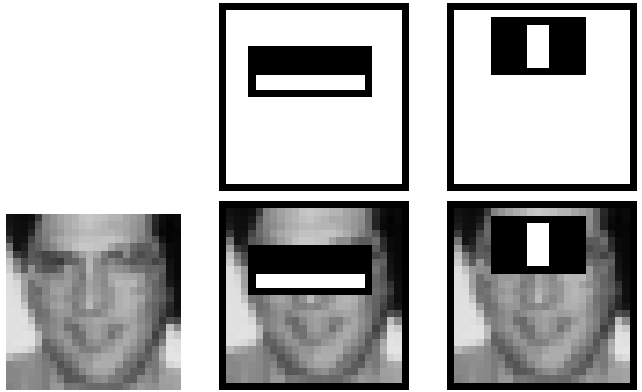
\includegraphics[scale=.4]{figs/top-features.png}
    \legend{Fonte: \citeauthoronline{paper-viola-jones} (\citeyear{paper-viola-jones})}
    \label{fig:top-features}
 \end{figure}

 A figura \ref{fig:top-features} retrata as melhores características registradas por \citeauthoronline{paper-viola-jones} (\citeyear{paper-viola-jones}), fica claro que as mesmas se destacam por evidenciar as regiões dos olhos e do nariz.

%-
\subsection{Classificador em Cascata}
%-

Pensando que, na maioria dos casos, uma face não ocupa a maior parte de uma imagem a ser identificada, é necessário encontrar uma forma rápida de descartar os elementos do fundo da mesma e concentrar o poder de processamento nos elementos que tem maior probabilidade de serem reconhecidos como uma face, isso leva a uma formulação para o problema onde ao contrário de encontrar faces, é necessário um algoritmo que descarte as "não faces".

Para tal problema, o classificador em cascata apresenta uma ótima solução, esta consiste na utilização de uma série de classificadores que são aplicados de forma sequencial, conforme ilustrado na imagem \ref{fig:cascade-classifier}, permitindo que imagens que certamente não possuem faces sejam rapidamente descartadas logo nas primeiras iterações, enquanto imagens com possíveis faces são classificadas por toda cascata, trazendo um elevado nível de confiança ao resultado.

\begin{figure}[htb]
    \centering
    \caption{Diagrama do funcionamento do classificador em cascata.}
    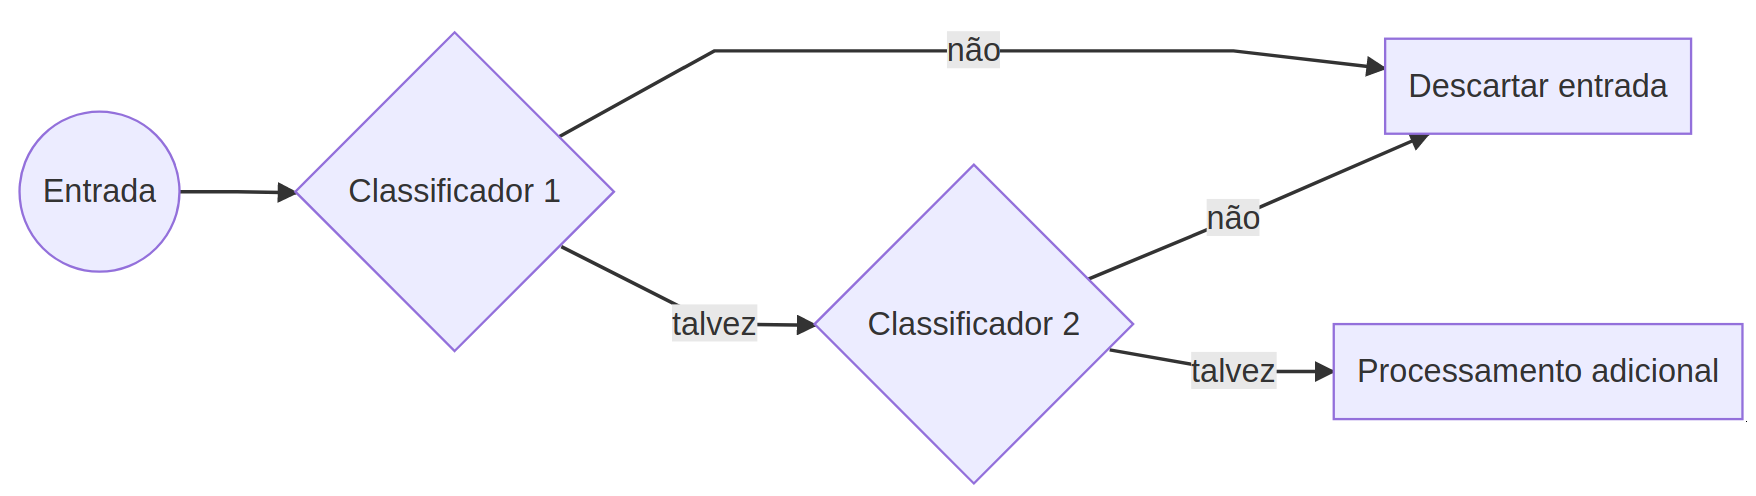
\includegraphics[scale=.2]{figs/cascade-classifier.png}
    \legend{Fonte: \citeauthoronline{paper-viola-jones} (\citeyear{paper-viola-jones})}
    \label{fig:cascade-classifier}
 \end{figure}

 Um classificador comum, com um único estágio normalmente aceitaria muitos casos de falso negativo, para reduzir a taxa de falsos positivos e de descarte de imagens relevantes, mas no classificador em cascata, falsos positivos nos primeiros estágios não são um problema, pois serão analisados em outros diversos estágios e provavelmente eliminados.

 A utilização desse modelo combinada com o algoritmo \textit{AdaBoost}, possibilita a análise das característica mais eficientes logo no início e consequentemente o descarte muito mais rápido dos casos negativos nos primeiros estágios.

 \section{Conjuntos de imagens para teste}

 Para analisar a eficiência da implementação do algoritmo \textit{Viola-Jones} na biblioteca \textit{OpenCV}, assim como o seu modelo previamente treinado, foram utilizados dois conjuntos de imagens. Tendo em mente o objetivo deste projeto, de identificar rapidamente imagens que não possuem uma face, são tratadas como imagens \textbf{positivas} as imagens que \textbf{não possuem faces} e como \textbf{negativas} as imagens que \textbf{possuem ao menos uma face}.

O primeiro dataset, nomeado \textit{Hotels-50k} \cite{hotels50k-article}, será utilizado para representar imagens \textbf{positivas}, portanto consiste em um conjunto de mais de 50 mil imagens de diversos quartos de hotel vazios, pois imagens com características semelhantes a estas são muitas vezes submetidas erroneamente em cadastros pessoais, ao invés de uma imagem da face a ser cadastrada.

O segundo dataset, nomeado \textit{UTKFace}, disponível em \citeonline{utkface}, será utilizado para representar imagens \textbf{negativas}, portanto consiste em um conjunto de mais de 20 mil imagens, com uma única face em cada, de diversas pessoas entre 0 e 116 anos de idade, catalogadas de acordo com idade, raça e sexo, alguns exemplos das imagens contidas no dataset podem ser vistos na figura \ref{fig:exemplos-utk}.

\begin{figure}[htb]
    \centering
    \caption{Exemplos de imagens do dataset \textit{UTKFace}.}
    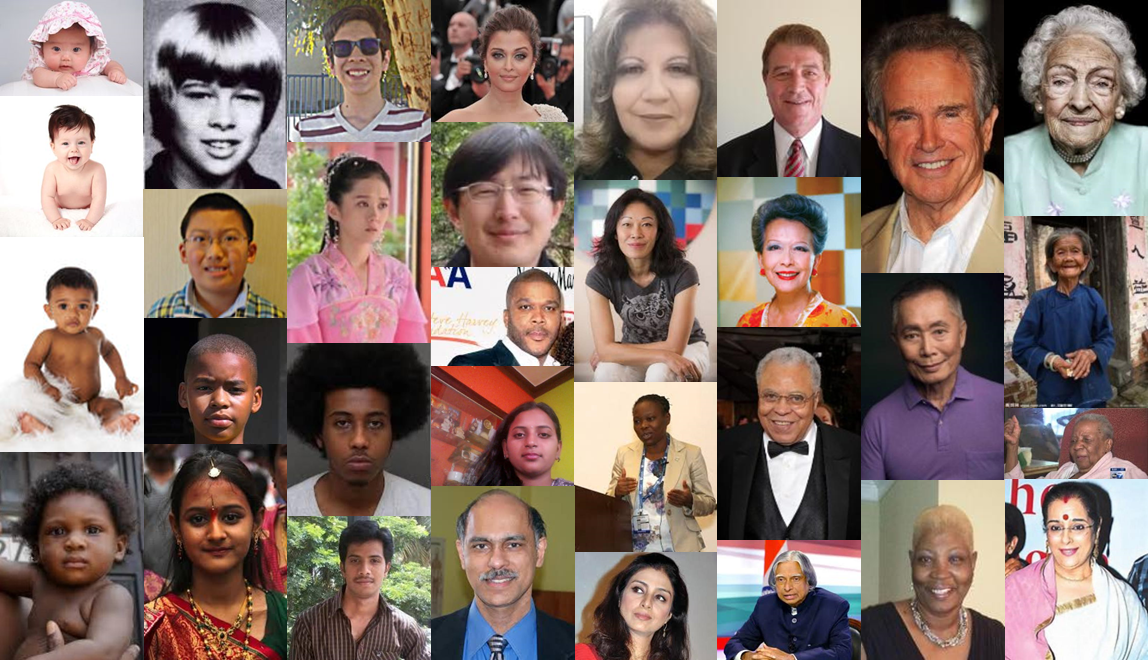
\includegraphics[scale=.3]{figs/exemplos-utk.png}
    \legend{Fonte: \textit{UTKFace dataset} \cite{utkface})}
    \label{fig:exemplos-utk}
 \end{figure}

 Para os testes, foram selecionadas aleatoriamente 17130 do dataset \textit{Hotels-50k} e selecionadas outras 17130 imagens do dataset \textit{UTKFace}, mas sendo essas apenas imagens de pessoas entre 18 e 60 anos de idade. Assim, foi totalizado um conjunto de 34260, onde metade delas eram positivas (não possuiam faces) e a outra metade negativas (possuiam ao menos uma face).

% % PARTE
% \part{Parte Final}
\chapter{Resultados e Discussão}\label{cap:resultados}

Após entender o funcionamento dos algoritmos e definir a metodologia para análise, foram executadas diversas iterações de classificação sobre o conjunto de imagens, variando os parâmetros de fator de escala (\textit{FE}) para e número mínimo de vizinhos (\textit{MV}), explicados anteriormente, e cada um dos resultados obtidos pode ser exibido como um ponto no espaço ROC obtendo a Figura \ref{fig:results_roc}, para que todos sejam facilmente comparados e também se torna simples observar se algum dos resultados está posicionado acima o limite lucrativo traçado.

\begin{figure}[htbp]
    \centering
    \caption{Resultados das classificações sobre o espaço ROC.}
    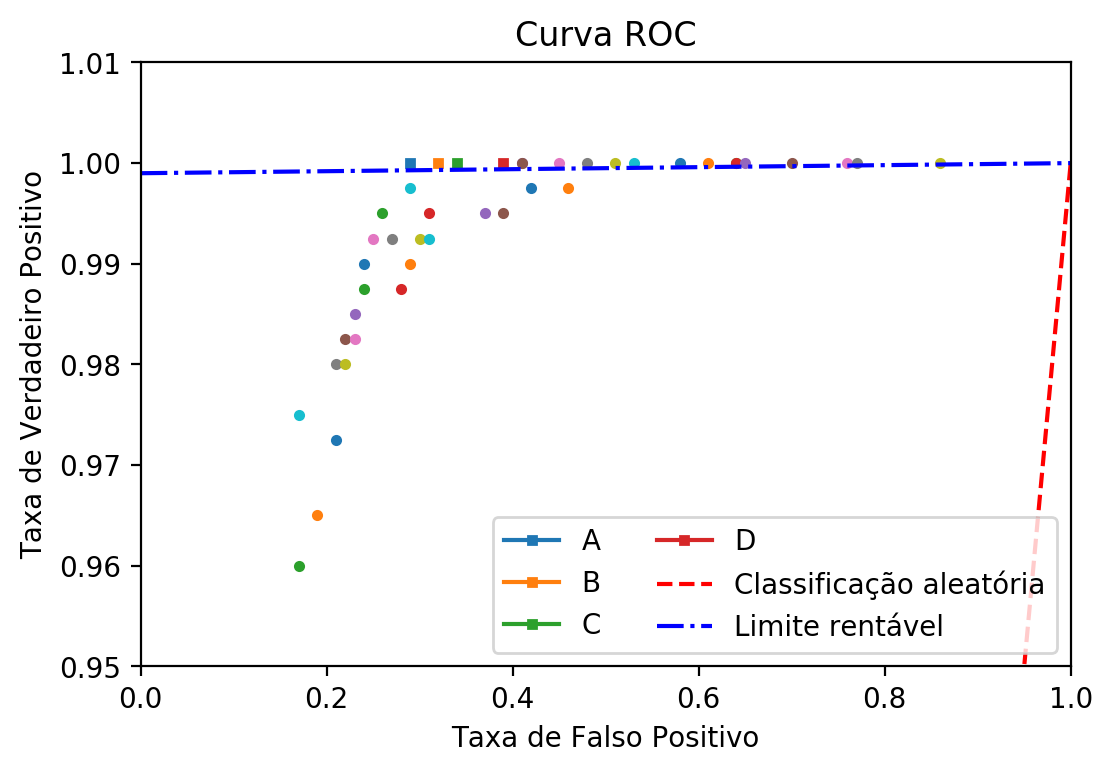
\includegraphics[scale=1]{figs/curva_roc_results.png}
    \legend{Os 4 resultados mais lucratívos são identificados por quadrados e o restante por círculos. Os parâmetros utilizados em cada resultado são listados na Tabela \ref{tab:results_identify}.}
    \label{fig:results_roc}
\end{figure}

\begin{table}[htbp]
    \caption{Resultados obtidos com os classificadores.\\$^1$Lucro refere-se ao lucro obtido por imagem analisada.}
    \label{tab:results_identify}
    \centering
    \begin{tabular}{clrrrrrr}
        Letra & Método & FE   & MV & Sensitividade & Especificidade & Acurácia & Lucro$^1$  \\
        \midrule
        A     & Keras  & -    & -  & 100,00\%      & 71,00\%        & 94,20\%  & R\$ 0,142  \\
        B     & OpenCV & 1,10 & 4  & 100,00\%      & 68,00\%        & 93,60\%  & R\$ 0,136  \\
        C     & OpenCV & 1,30 & 1  & 100,00\%      & 66,00\%        & 93,20\%  & R\$ 0,132  \\
        D     & OpenCV & 1,10 & 3  & 100,00\%      & 61,00\%        & 92,20\%  & R\$ 0,122  \\
        E     & OpenCV & 1,25 & 1  & 100,00\%      & 59,00\%        & 91,80\%  & R\$ 0,118  \\
        -     & OpenCV & 1,05 & 5  & 100,00\%      & 59,00\%        & 91,80\%  & R\$ 0,118  \\
        -     & OpenCV & 1,05 & 4  & 100,00\%      & 55,00\%        & 91,00\%  & R\$ 0,110  \\
        -     & OpenCV & 1,10 & 2  & 100,00\%      & 52,00\%        & 90,40\%  & R\$ 0,104  \\
        -     & OpenCV & 1,15 & 1  & 100,00\%      & 49,00\%        & 89,80\%  & R\$ 0,098  \\
        -     & OpenCV & 1,05 & 3  & 100,00\%      & 47,00\%        & 89,40\%  & R\$ 0,094  \\
        -     & OpenCV & 1,10 & 1  & 100,00\%      & 42,00\%        & 88,40\%  & R\$ 0,084  \\
        -     & OpenCV & 1,05 & 2  & 100,00\%      & 39,00\%        & 87,80\%  & R\$ 0,078  \\
        -     & OpenCV & 1,30 & 0  & 100,00\%      & 36,00\%        & 87,20\%  & R\$ 0,072  \\
        -     & OpenCV & 1,25 & 0  & 100,00\%      & 36,00\%        & 87,20\%  & R\$ 0,072  \\
        -     & OpenCV & 1,20 & 0  & 100,00\%      & 35,00\%        & 87,00\%  & R\$ 0,070  \\
        -     & OpenCV & 1,05 & 1  & 100,00\%      & 30,00\%        & 86,00\%  & R\$ 0,060  \\
        -     & OpenCV & 1,15 & 0  & 100,00\%      & 24,00\%        & 84,80\%  & R\$ 0,048  \\
        -     & OpenCV & 1,10 & 0  & 100,00\%      & 23,00\%        & 84,60\%  & R\$ 0,046  \\
        -     & OpenCV & 1,05 & 0  & 100,00\%      & 14,00\%        & 82,80\%  & R\$ 0,028  \\
        -     & OpenCV & 1,10 & 5  & 99,75\%       & 71,00\%        & 94,00\%  & -R\$ 0,356 \\
        -     & OpenCV & 1,15 & 2  & 99,75\%       & 58,00\%        & 91,40\%  & -R\$ 0,382 \\
        -     & OpenCV & 1,20 & 1  & 99,75\%       & 54,00\%        & 90,60\%  & -R\$ 0,390 \\
        -     & OpenCV & 1,10 & 6  & 99,50\%       & 74,00\%        & 94,40\%  & -R\$ 0,848 \\
        -     & OpenCV & 1,20 & 2  & 99,50\%       & 69,00\%        & 93,40\%  & -R\$ 0,858 \\
        -     & OpenCV & 1,15 & 3  & 99,50\%       & 63,00\%        & 92,20\%  & -R\$ 0,870 \\
        -     & OpenCV & 1,05 & 6  & 99,50\%       & 61,00\%        & 91,80\%  & -R\$ 0,874 \\
        -     & OpenCV & 1,30 & 2  & 99,25\%       & 75,00\%        & 94,40\%  & -R\$ 1,344 \\
        -     & OpenCV & 1,15 & 5  & 99,25\%       & 73,00\%        & 94,00\%  & -R\$ 1,348 \\
        -     & OpenCV & 1,15 & 4  & 99,25\%       & 70,00\%        & 93,40\%  & -R\$ 1,354 \\
        -     & OpenCV & 1,25 & 2  & 99,25\%       & 69,00\%        & 93,20\%  & -R\$ 1,356 \\
        -     & OpenCV & 1,15 & 6  & 99,00\%       & 76,00\%        & 94,40\%  & -R\$ 1,840 \\
        -     & OpenCV & 1,20 & 3  & 99,00\%       & 71,00\%        & 93,40\%  & -R\$ 1,850 \\
        -     & OpenCV & 1,20 & 4  & 98,75\%       & 76,00\%        & 94,20\%  & -R\$ 2,338 \\
        -     & OpenCV & 1,25 & 3  & 98,75\%       & 72,00\%        & 93,40\%  & -R\$ 2,346 \\
        -     & OpenCV & 1,30 & 3  & 98,50\%       & 77,00\%        & 94,20\%  & -R\$ 2,834 \\
        -     & OpenCV & 1,20 & 5  & 98,25\%       & 78,00\%        & 94,20\%  & -R\$ 3,330 \\
        -     & OpenCV & 1,25 & 4  & 98,25\%       & 77,00\%        & 94,00\%  & -R\$ 3,332 \\
        -     & OpenCV & 1,25 & 5  & 98,00\%       & 79,00\%        & 94,20\%  & -R\$ 3,826 \\
        -     & OpenCV & 1,20 & 6  & 98,00\%       & 78,00\%        & 94,00\%  & -R\$ 3,828 \\
        -     & OpenCV & 1,25 & 6  & 97,50\%       & 83,00\%        & 94,60\%  & -R\$ 4,814 \\
        -     & OpenCV & 1,30 & 4  & 97,25\%       & 79,00\%        & 93,60\%  & -R\$ 5,320 \\
        -     & OpenCV & 1,30 & 5  & 96,50\%       & 81,00\%        & 93,40\%  & -R\$ 6,810 \\
        -     & OpenCV & 1,30 & 6  & 96,00\%       & 83,00\%        & 93,40\%  & -R\$ 7,802 \\
    \end{tabular}
\end{table}

Analisando os resultados de sensitividade, especificidade e acurácia de cada um dos classificadores na Tabela \ref{tab:results_identify} e a matriz de confusão do resultado que mais lucrativo na Tabela \ref{tab:matriz_de_confusao_best_result}, é possível obter algumas conclusões interessantes.

\begin{table}[htbp]
    \caption{Matriz de confusão com os resultados do classificador mais lucrativo.}
    \label{tab:matriz_de_confusao_best_result}
    \centering
    \begin{tabular}{cccc}\hline\hline
                       & \textit{B} & $\overline{B}$ & Soma  \\
        \textit{A}     & 80.0\%     & 00.0\%         & 80\%  \\
        $\overline{A}$ & 05.8\%     & 14.2\%         & 20\%  \\
        Soma           & 85.8\%     & 14.2\%         & 100\% \\
        \hline\hline
    \end{tabular}
\end{table}

Comparando tal resultado com a análise da equação que define o limiar lucrativo da classificação, é possível perceber que cada imagem positiva que é classificada como negativa gera um prejuízo muito elevado, que precisa ser compensado com a classificação correta de uma grande quantidade de imagens negativas. Para o classificador estudado, percebe-se que todos os cenários lucrativos apresentam sensitividade igual a 100\%, ou seja, todas imagens positivas foram classificadas corretamente.

É curioso notar que o lucro não é diretamente proporcional a acurácia do detector, destacando que a configuração de maior acurácia apresentou prejuízo, tal fato também ocorre devido ao prejuízo elevado de classificar uma imagem positiva de forma incorreta.
\chapter{Conclusões e Trabalhos Futuros}\label{cap:conclusao}

\section{Conclusões}

Relembrando o objetivo do projeto, que consiste em negar rapidamente imagens que certamente não possuem nenhuma face, e observando os resultados obtidos e análisados, pode-se concluir que tanto o algoritmo de Viola-Jones quanto o MTCNN poderiam ser utilizado de forma satisfatória para solucionar tal problema, mesmo utilizando um modelo já treinado, desde que parametrizados da forma correta, permitindo a obtenção lucros de alguns centavos por imagem, que em grande escala (milhares de imagens) pode ser relevante para uma empresa.

Durante o desenvolvimento do projeto foi possível perceber que o ajuste fino de um modelo tem grande impacto no seu resultado final, podendo ser considerada a parte mais importante para um projeto de implementação de um sistema de detecção facial.

Além disso, os testes apenas apresentaram resultados positivos após a seleção correta do conjunto de imagens, o que é um forte indicativo de que o modelo precisa ser preparado especificamente para as necessidades existentes.

\section{Trabalhos Futuros}

Para dar continuidade ao desenvolvimento desse projeto, podem ser estudadas outras metodologias de detecção facial ou evoluções da metodologia utilizada, adicionando técnicas como corte e rotação das imagens originais, que permitiriam ao classificador ser mais específico, por trabalhar com imagens melhor padronizadas.

Além disso, dada a necessidade apresentada, em que as imagens devem cumprir algumas características específicas além de apenas conter uma face, torna-se interessante a busca por um conjunto maior de imagens que permitiria o treinamento de um modelo específico para tal problema, que deve apresentar resultados ainda melhores.


% ----------------------------------------------------------
% ELEMENTOS PÓS-TEXTUAIS (Referências, Glossário, Apêndices)
% ----------------------------------------------------------
\postextual

% Referências bibliográficas
\bibliography{bibliografia}

% Glossário (Consulte o manual)
%\glossary

% % Apêndices
% % ----------------------------------------------------------
% Apêndices
% ----------------------------------------------------------

% ---
% Inicia os apêndices
% ---
\begin{apendicesenv}

% Imprime uma página indicando o início dos apêndices
\partapendices

% ----------------------------------------------------------
\chapter{Primeiro Apêncice}
% ----------------------------------------------------------

\lipsum[50] % Texto qualquer. REMOVER!!

% ----------------------------------------------------------
\chapter{Segundo apêndice com título tão grande quanto se queira porque ele já faz a quebra de linha da coisa toda}
% ----------------------------------------------------------
\lipsum[51-53] % Texto qualquer. REMOVER!!

\end{apendicesenv}
% ---

% % Anexos
% % ----------------------------------------------------------
% Apêndices
% ----------------------------------------------------------

% ---
% Inicia os anexos
% ---
\begin{anexosenv}

% Imprime uma página indicando o início dos anexos
\partanexos

% ---
\chapter{Nome do Primeiro Anexo}
% ---
\lipsum[30] % Texto qualquer. REMOVER!!

% ---
\chapter{Nome de Outro Anexo}
% ---

\lipsum[32] % Texto qualquer. REMOVER!!

\end{anexosenv}

% Índice remissivo (Consultar manual)
%\phantompart
%\printindex

\end{document}
